\section{Introduction}
    As technology becomes more advanced those who design, use, and are affected by it in other ways want to know that it will perform correctly, and understand why it does what is does, and how to use it appropriately. In essence people who interact with advanced technology want to be able to trust it appropriately, and then act on that trust.

    In interpersonal relationships, and otherwise, humans act based on trust. For example a supervisor asks a subordinate to accomplish a task based on several factors that indicate they can trust them to accomplish that task. When consumers make purchases they do so with trust that the product will perform as promised. Likewise, when using something like an autonomous vehicle the user must be able to trust it appropriately in order to use it properly. \textbf{I really don't like this paragraph much, but I'll have to come back later}.

    With the rapid advancement of the capabilities of computing technology to do tasks that were previously assumed to be too complicated for computers, there has been much recent discussion regarding how humans can trust this technology -- if not always explicitly stated as such. This discussion has taken place both in public \cite{Spectrum2016-jv,DeSteno2014-cq,Cranz2017-yh,Cassel2017-tn,Danks_undated-sb}, corporate \cite{Banavar2016-nm, Khosravi2016-ke,Moody2017-vd,Rudnitsky2017-in,Benioff2016-tc}, and academic \cite{Groom2007-bz,Lloyd_undated-bb,Goodrum_2016-fm,Foley2017-qj,Ghahramani2015-yq,Castelvecchi2016-mr} settings.

    Specifically, in this survey, I investigate what assurances an Artificially Inteligent Agent (AIA) can provide to a human user in order to affect their trust. The colloquial definitions of `appropriate use', `assurance', `AIA', and `trust' should suffice for now to give the reader a general idea of the motivation; more formal definitions will be presented in section \ref{sec:background}.

    Figure \ref{fig:SimpleTrust_one_way} is a simple diagram of the trust cycle that exists between a human user and an AIA (justification for the existence of this cycle will be presented later). Simply, the user's trust is affected by assurances that in turn affect the user's behaviors (e.g. trust AIA with responsibilities, or not).

    \begin{figure}
        \centering
        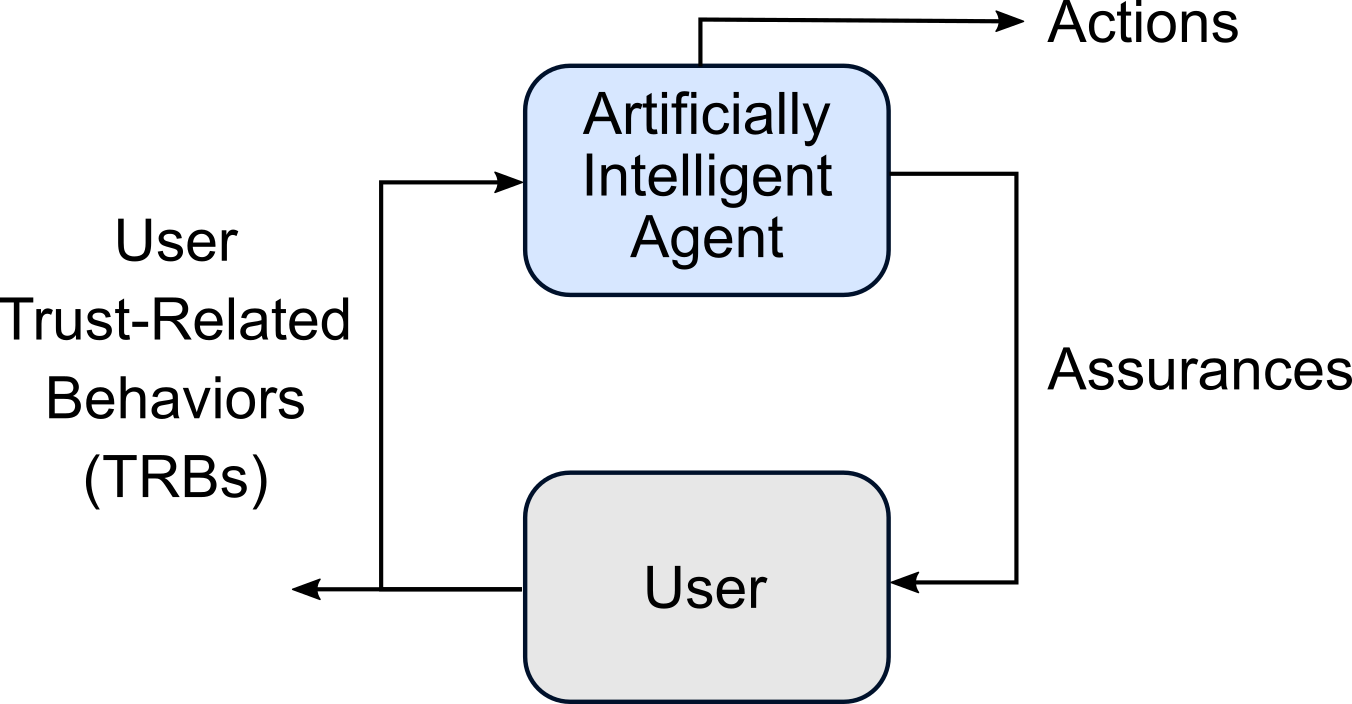
\includegraphics[width=0.5\textwidth]{Figures/SimpleTrust_one_way.png}
        \caption{Diagram depicting the simple one-way trust relationship between a human user and an AIA. Based on a user's level of trust they take certain actions (e.g. give AIA commands), these commands can lead the AIA to certain actions and/or to provide assurances to the user in order to affect their trust.}
        \label{fig:SimpleTrust_one_way}
    \end{figure}

    In order to understand assurances, one must have a more formal understanding of each term in figure \ref{fig:SimpleTrust_one_way}. This because the cycle is serial, and is not complete with a missing component. To this end, section \ref{sec:background} provides definitions for each of the terms. In section \ref{sec:methodology} I discuss the methodology I used when compiling this survey. Afterwards, section \ref{sec:survey} will discuss the current landscape of assurances that exist in the literature. Finally, section \ref{sec:conclusions} contains some last discussion and conclusions.
